\documentclass[tikz,margin=5pt]{standalone}
\usepackage{tikz}
\usepackage{pgfplots}
\pgfplotsset{compat=1.16}

\usepackage{graphicx}

%\usepackage{newtxtext}
%\usepackage{newtxmath}
\usepackage{mathpazo}

\begin{document}
\begin{tikzpicture}
  \node[above] at (0,0) {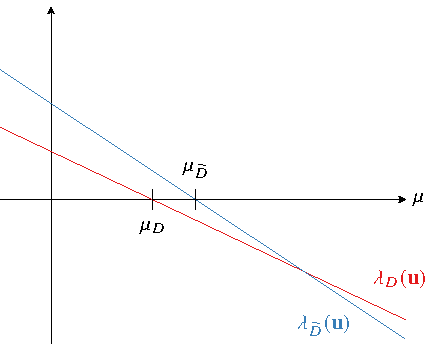
\includegraphics[scale=0.8]{eigenplot1.pdf}};
  \node[above] at (6.5,0) {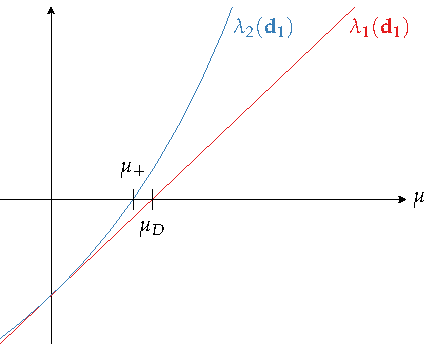
\includegraphics[scale=0.8]{eigenplot2.pdf}};

  \node[above] at (-2.8,5) {\textbf{A}};
  \node[above] at (-2.8 + 6.5,5) {\textbf{B}};
\end{tikzpicture}
\end{document}

